% Standalone experimental-plan doc (renders on its own, like Previous_Work).
% Figures live in figures/experiments/ relative to this file, so compile from
% within paper/.  To fold into the main manuscript instead, delete the preamble
% and the \begin{document}/\end{document}/\maketitle lines and \input the rest.
\documentclass{article}
\usepackage[margin=1in]{geometry}
\usepackage{amsmath}
\usepackage{graphicx}
\usepackage{booktabs}
\usepackage{enumitem}
\usepackage{hyperref}
\hypersetup{colorlinks=true, linkcolor={blue!90!black!70}}

\setlength{\parskip}{4pt}
\setlength{\parindent}{0pt}
\setlist{nosep, leftmargin=1.4em}

\title{Experimental Plan: Sparsified Composite Subsampling}
\date{}

\begin{document}
\maketitle

\paragraph{Setting.} Inductive, node-level DP:
\begin{itemize}
  \item Train on the train-induced subgraph; test on held-out nodes absent at training.
  \item Transductive training is privacy-sound (Theorem~6.4 substitutes any node, so test nodes are covered too) but its test accuracy does not measure generalization to unseen nodes; we report both settings.
  \item Inductive $\Rightarrow$ guarantee covers exactly the training nodes; test accuracy is honest.
  \item Sparsification ($p_1$ roots, $p_2$/$r$ edges) is unchanged by this choice.
\end{itemize}

\paragraph{Orientation.} Expansion follows \emph{incoming} edges
(\textsc{SparseExpand}$_{\mathrm{in}}$, Algorithm~5): a message-passing GNN builds
the root's representation from vertices admitting a directed path \emph{to} it.
Under the earlier out-oriented expansion every retained arc left the root on the
source side, so during training the root's representation was bit-identical to
that of an isolated node and the per-root loss was a graph-blind MLP loss. All
runs therefore use \texttt{--direction in}; \texttt{--direction out} is retained
only for the ablation, and any number recorded before this fix is not comparable.

\paragraph{Protocol.}
\begin{itemize}
  \item Base mechanism $g_0$: two-layer GCN, one loss per sampled root on its rooted subgraph.
  \item Baseline: same engine, graph-blind MLP (root features only, $r{=}0$).
  \item Cap in/out degree at $K_{\mathrm{in}},K_{\mathrm{out}}$ (Assumption~6.2).
  \item Clip each per-root gradient to $\|g_0\|_2\le C$, add $\mathcal N(0,(\sigma C)^2 I)$.
  \item Accounting is post-hoc at $\delta$ via Theorem~6.4 (node substitution),
        whose shells are $n_d=K_{\mathrm{out}}^d$ --- so for in-expansion it is the
        \emph{out}-degree cap that prices the guarantee.
\end{itemize}

\paragraph{Ladder.} Each stage isolates one effect:
\begin{enumerate}
  \item[\textbf{S0}] Baselines, no DP: MLP; full-edge GCN (utility ceiling).
  \item[\textbf{S1}] Sparsification only, no DP: sweep $p_2,r$ on the capped graph.
  \item[\textbf{S2}] Add clip + noise: at the S1 config, sweep $\sigma$.
  \item[\textbf{S3}] Accounting: attach Theorem~6.4 $\varepsilon$ to S2 (privacy--utility frontier).
\end{enumerate}

\paragraph{Sweep.}
$p_1$ fixed (batch $\approx p_1\lvert V_{\mathrm{train}}\rvert$);
$p_2\in\{0.1,0.25,0.5,1.0\}$; $r\in\{1,2\}$;
$K_{\mathrm{in}}{=}K_{\mathrm{out}}\in\{5,10\}$; $\sigma\in\{2,5,10,20\}$;
$C{=}1$; $\delta{=}10^{-6}$; $\ge 3$ seeds.

\paragraph{Datasets.}
\begin{itemize}
  \item Homogeneous inductive first: ogbn-arxiv (temporal split), Flickr, Reddit.
  \item Disjoint-graph (cleanest node-DP): PPI --- the 24 graphs are split 20/2/2,
        so training expansion cannot reach a held-out node at any $r$, with no
        train-induced-subgraph surgery. Multilabel, so micro-F1.
  \item RelBench entity tasks (temporal, natively inductive; AUROC). A root is one
        prediction row, reaching its entity at $r{=}1$ and that entity's history at
        $r{=}2$. rel-f1 validates the pipeline but has only $1353$ training rows;
        the $\varepsilon$ numbers come from rel-stack / rel-hm.
\end{itemize}

\paragraph{Pilot: ogbn-arxiv (inductive), S0--S1.} $p_1{=}0.005$, $K{=}5$, $T{=}500$, 3 seeds (Table~\ref{tab:plan-arxiv}, Fig.~\ref{fig:plan-ladder}).
\emph{Superseded: Table~\ref{tab:plan-arxiv} and Fig.~\ref{fig:plan-ladder} were
produced with out-oriented expansion and are being regenerated.} Under
re-measurement at $2$ seeds the two orientations are statistically
indistinguishable on this graph ($0.520$ vs.\ $0.519$ test accuracy, $\pm 0.02$),
both about three points above the MLP: capping to $K_{\mathrm{in}}{=}K_{\mathrm{out}}{=}5$
erases arxiv's degree asymmetry, and evaluation always propagated along incoming
edges, so out-oriented training was a train/eval mismatch rather than an outright
graph-blind pipeline. The earlier qualitative claims survive:
\begin{itemize}
  \item Degree cap is free: in-degree $3015\!\to\!5$ (drops $88\%$ of edges) matches the full-edge ceiling.
  \item Sparsification nearly free: $p_2$ $1.0\!\to\!0.1$ loses under two points.
  \item Depth doesn't help: $r{=}2$ does not beat $r{=}1$.
\end{itemize}

\begin{table}[htbp]
  \centering\footnotesize
  \caption{ogbn-arxiv, inductive, no DP (test accuracy, mean$\pm$sd over 3 seeds).}
  \label{tab:plan-arxiv}
  \begin{tabular}{lcc}
    \toprule
    Model & Config & Test acc \\
    \midrule
    MLP (graph-blind) & $r{=}0$          & $0.488 \pm 0.011$ \\
    GCN ceiling       & full edges, $r{=}2$ & $0.518 \pm 0.011$ \\
    \midrule
    GCN, $K{=}5$, $r{=}1$ & $p_2{=}1.0$  & $0.519 \pm 0.003$ \\
    GCN, $K{=}5$, $r{=}1$ & $p_2{=}0.5$  & $0.509 \pm 0.005$ \\
    GCN, $K{=}5$, $r{=}1$ & $p_2{=}0.25$ & $0.500 \pm 0.002$ \\
    GCN, $K{=}5$, $r{=}1$ & $p_2{=}0.1$  & $0.504 \pm 0.007$ \\
    \bottomrule
  \end{tabular}
\end{table}

\paragraph{Orientation ablation.} The observation that out-expansion gives
$\sim\!1.6$ neighbors on arxiv at $p_2{=}1$ (Fig.~\ref{fig:plan-ladder}, bottom)
was the symptom that prompted Sections~5--6. Running one configuration at each
orientation is now an experiment in its own right
(\texttt{scripts/orientation\_ablation.sh}):
\begin{itemize}
  \item \textbf{Utility.} Only in-expansion delivers neighbor features to the
        root during training. On arxiv the gap sits inside the seed noise once
        degrees are capped ($3015,221 \to 5,5$ erases the asymmetry), but it is
        decisive on RelBench, where the corrected orientation moves
        rel-f1/driver-top3 from chance to $0.79$ AUROC.
  \item \textbf{Privacy.} Reported as \texttt{epsilon\_substitution}, computed for
        both orientations and so comparing like with like: in-expansion pays
        $n_d{=}K_{\mathrm{out}}^d$ and out-expansion $n_d{=}K_{\mathrm{in}}^d$, so
        the cheaper orientation is whichever direction the graph is thin in. Under
        $K_{\mathrm{in}}{=}K_{\mathrm{out}}$ the two coincide exactly.
  \item \textbf{Adjacency notion.} The tighter insertion/removal pair
        (Theorem~4.5, sensitivity $C$ rather than $2C$) exists only for
        out-expansion, so it is an ablation rather than the headline. Its shells
        activate all-or-nothing, which at the small $p_1$ used here makes it
        \emph{looser} than Theorem~6.4 despite the better sensitivity: on the
        arxiv grid ($p_1{=}0.005$, $K{=}5$, $r{=}1$, $T{=}500$, $\sigma{=}10$,
        $p_2{=}0.1$) it gives $\varepsilon{=}7.2$ where the substitution pair
        gives $0.51$.
\end{itemize}

\paragraph{RelBench specifics.} The relational graph is built from the raw
database: one node per row, one arc per foreign key oriented child~$\to$~parent,
and one arc entity~$\to$~prediction-row, so information flows
results~$\to$~driver~$\to$~row and in-expansion from a row root walks its entity's
history. Splits are temporal; training expands over the graph as of the train
cutoff while evaluation uses the full graph. Here $K_{\mathrm{out}}$ is the knob
that decides whether $\varepsilon$ is finite at all, since an entity feeds one arc
per prediction row: on rel-f1 at $p_1{=}0.05$, $r{=}2$, $\sigma{=}5$, $T{=}300$,
$\varepsilon$ runs $33.3,\,78.1,\,287,\,2185,\,\infty$ for
$K_{\mathrm{out}}{=}2,3,5,10,20$. It is swept, not fixed.

\begin{figure}[htbp]
  \centering
  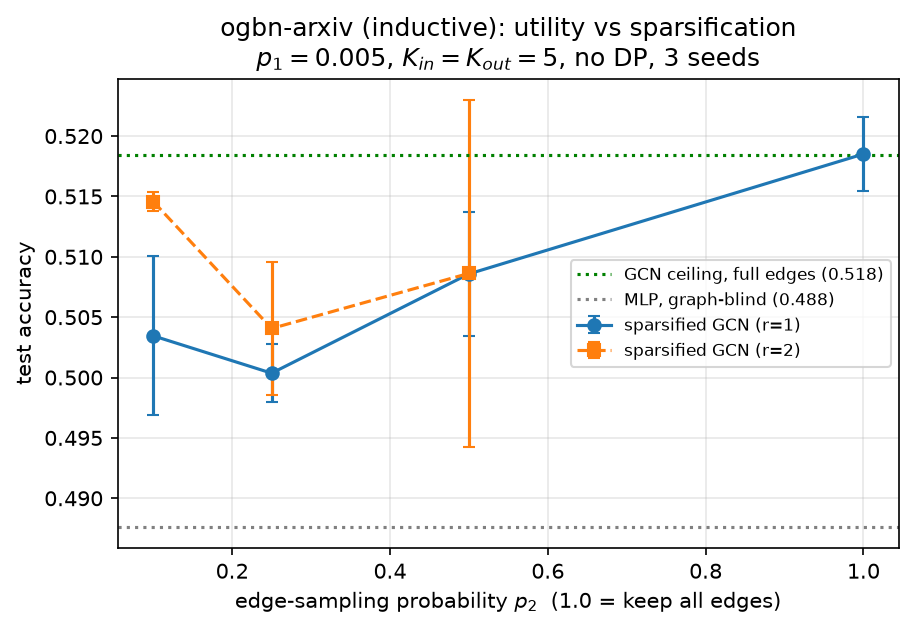
\includegraphics[width=0.72\linewidth]{figures/experiments/inductive_ladder.png}\\[6pt]
  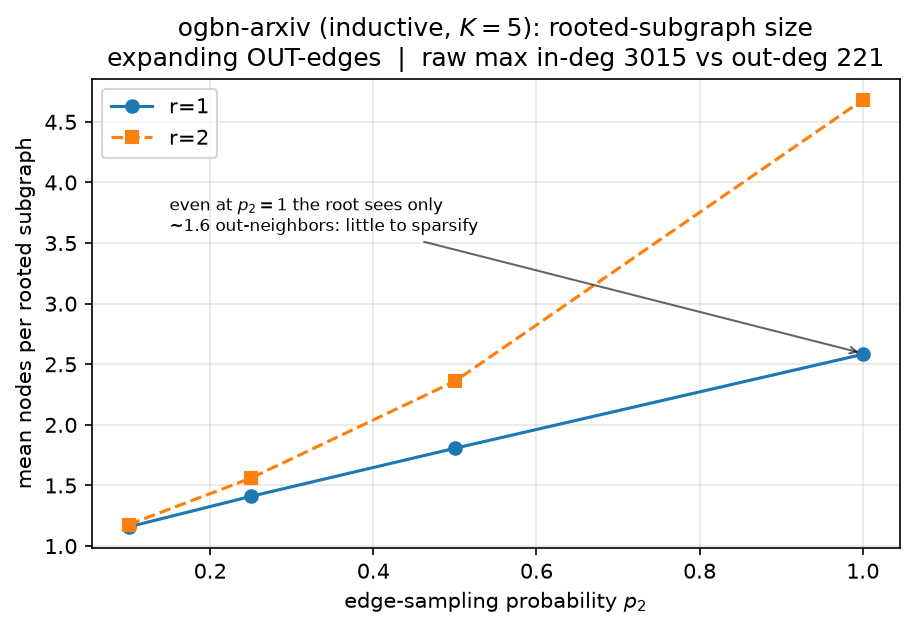
\includegraphics[width=0.72\linewidth]{figures/experiments/inductive_subgraph_size.png}
  \caption{Top: utility vs.\ $p_2$; the sparsified family sits between the MLP
    and the full-edge ceiling. Bottom: rooted-subgraph size --- out-neighborhoods
    stay tiny, explaining the flat ladder.}
  \label{fig:plan-ladder}
\end{figure}

\end{document}
